\section{Batch processing tool based on C}

\subsection{Disassembly}
The C-Binary was optained by downloading it from the VM. We used \code{IDA PRO Free} to disassemple the binary code.
We found out, that the file was composed in two important functions: The \code{main}-function and the function \code{mysql\_query\_function}. In the \code{main}-function the input text file gets parsed and in a loop the \code{mysql\_query\_function}-function gets called to make the changes in the database and apply the transactions.
We used the flow diagram and disassebled code generated by \code{IDA PRO Free} to reconstruct the C-code the binary was generated from.

\subsection{Analysis of Working}
\begin{itemize}
\item Using the original binary with the provided test file does not work and exists with \enquote{Negative transactions not allowed}
\item All query executions are vulnerable to SQL-Injection.
\item The application repeatedly uses \code{strcpy()} and \code{strcat()} without length checks. This makes it vulnerable to buffer overflow attacks.
\item SQL credentials are included in the binary in plain text. See \ref{fig:ida_db_info2}.
\end{itemize}

\begin{figure}[ht]
	\centering
	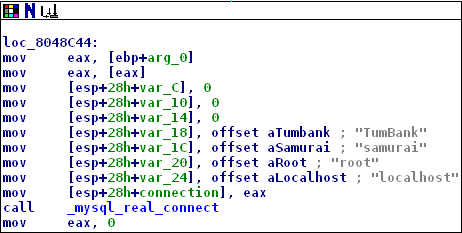
\includegraphics[width=.8\linewidth]{figures/ida_db_info.png}
	\caption{IDA PRO Free: Extracted Secrets}
	\label{fig:ida_db_info2}
\end{figure}